\section*{Choices of activation function}

    Our linear model is entirely \textbf{defined} by its input: the number of \textbf{weights} in a neuron is just the number of \textbf{inputs} $m$.
    
    But our \textbf{activation} function is up to us to decide: what works best?
    
    \subsection*{Trying out linear activation}
        
        The simplest assumption would be to just use the \textbf{identity} function 
        
        \begin{equation}
            f(z) = z
        \end{equation}
        
        We might hope that we can combine a bunch of simple, \textbf{linear} models, and get a more sophisticated model. Why bother having a \textbf{nonlinear} activation at all?
        
        Well, it turns out, combining \textbf{multiple} linear layers doesn't make our model any stronger. Let's try an example: we'll take a network with 2 layers, two neurons each.
        
        Let's look at layer 1: 
        
        \begin{figure}[H]
            \centering
            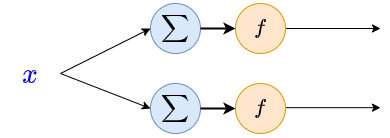
\includegraphics[width=70mm,scale=0.4]{images/nn_images/layer_one_linear.png}
        \end{figure}
        
        Since the activation function has \textbf{no effect} on our result, we can \textbf{omit} it:
        
        \begin{figure}[H]
            \centering
            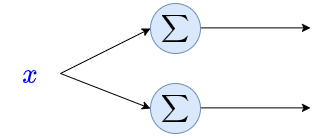
\includegraphics[width=70mm,scale=0.4]{images/nn_images/linear_layer_omitted.png}
        \end{figure}
        
        And now, we can show our \textbf{full} network:
        
        \begin{figure}[H]
            \centering
            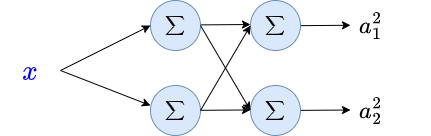
\includegraphics[width=70mm,scale=0.4]{images/nn_images/two_layers_linear.png}
        \end{figure}
        
    \subsection*{Linear Layers: An example}
        
        We'll assume \textbf{two} inputs $A_0 = [x_1, x_2]^T$. For our sanity, we'll lump all of the weights in each \textbf{layer}:
        
        \begin{figure}[H]
            \centering
            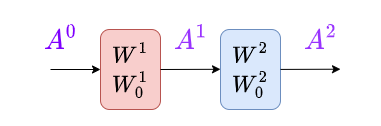
\includegraphics[width=70mm,scale=0.4]{images/nn_images/two_layer_linear_layer_view.png}
        \end{figure}
        
        We'll leave out $W_0$ terms to make it more readable, but the same will apply. 
        
        Layer 1:
        
        \begin{equation}
            A^1 = (\red{W^1})^T \pur{A_0} 
        \end{equation}
        
        Layer 2:
        
        \begin{equation}
            A^2 = 
            \overbrace{
            (\blu{W^2})^T (\red{W^1})^T
            }^{\text{Weight matrices}}
            \pur{A_0} 
        \end{equation}
        
        The full function for this equation is two matrices, \textbf{multiplied} by our input vector.
        
        Let's take an arbitrary example:
        
        \begin{equation}
            W^1 = 
            \red{
            \begin{bmatrix}
                1 & 2 \\ 3 & 4
            \end{bmatrix}
            }
            \qquad
            \blu{
            W^2 = 
            \begin{bmatrix}
                5 & 6 \\ 7 & 8
            \end{bmatrix}
            }
        \end{equation}
        
        Our equation becomes:
        
        \begin{equation}
            A^2 = 
            \overbrace{
                \blu{
                \begin{bmatrix}
                    5 & 7 \\ 6 & 8
                \end{bmatrix}
                }
                \red{
                \begin{bmatrix}
                    1 & 3 \\ 2 & 4
                \end{bmatrix}
                }
            }^{\text{Transposed matrices}}
            \pur{
            \begin{bmatrix}
                x_1 \\ x_2
            \end{bmatrix}
            }
        \end{equation}
        
        We created this function by applying two matrices separately. But, can't we \textbf{combine} them?
       
        \begin{equation}
            A^2 =
            \begin{bmatrix}
                19 & 43 \\ 22 & 50
            \end{bmatrix}
            \pur{
            \begin{bmatrix}
                x_1 \\ x_2
            \end{bmatrix}
            }
        \end{equation}
       
        Wait, but this looks like a \textbf{one-layer} network with those weights! The second layer is \textbf{pointless}, we could have represented it with a single layer...
       
        \begin{equation}
           (W^{12})^T = 
           \begin{bmatrix}
                19 & 43 \\ 22 & 50
            \end{bmatrix}
        \end{equation}
    
    \subsection*{The problem with linear networks}
    
        In fact, this is true in general: we can always take our \textbf{two} linear layers and combine them into \textbf{one}.
        
        \begin{equation}
            (\blu{W^2})^T (\red{W^1})^T
            = W^{12}
        \end{equation}
        
        Our network is \textbf{equivalent} to the supposedly "simpler" one-layer network.
    
        \begin{figure}[H]
            \centering
            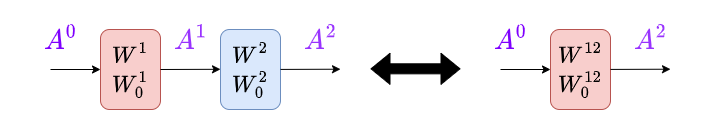
\includegraphics[width=80mm,scale=0.4]{images/nn_images/equivalent_networks.png}
        \end{figure}
        
        What if we have more layers? Well, we can just combine them one-by-one. At the end, we're just left with one layer:
        
        \begin{equation}
            (\pur{W^L})^T (\org{ {W^{L-1}} })^T \cdots (\blu{W^2})^T (\red{W^1})^T
            = W^{X}
        \end{equation}
        
        And so, we can't just use linear layers: we \textbf{need} a \textbf{nonlinear} activation function.\\
        
        \begin{concept}
            Having multiple consecutive \vocab{linear layers} (i.e. layers with linear \gren{activation} functions) is \purp{equivalent} to having one linear layer in its place.
            
            This means that we do not expand our \purp{hypothesis} class by using more linear layers: we have to use \gren{nonlinear} activation functions.
        \end{concept}
        
        If we use something \textbf{nonlinear}...
        
        \begin{equation}
            A^2 = 
            \org{f}
            \Bigg( 
                (\blu{W^2})^T 
                \red{A^1}
            \Bigg)
        \end{equation}
        
        We get something that doesn't \textbf{simplify}:
            \note{This is ugly, but we don't have to worry about the details.}
        
        \begin{equation}
            A^2 = 
            \org{f}
            \Bigg( 
                (\blu{W^2})^T 
                \overbrace{
                    \boxed{
                        \org{f}
                        \Big(
                            \red{ (W^1)^T x }
                        \Big)
                    }
                }^{A^1}
            \Bigg)
        \end{equation}
        
        Which is what we want!
        